\documentclass[rusmathsym, eqnumwithinsec, amspack, hyperref]{bomgost}

\DeclareTextSymbol{\CYRA}\UnicodeEncodingName{"0410}        % А
\DeclareTextSymbol{\cyra}\UnicodeEncodingName{"0430}        % а
\DeclareTextSymbol{\CYRB}\UnicodeEncodingName{"0411}        % Б
\DeclareTextSymbol{\cyrb}\UnicodeEncodingName{"0431}        % б
\DeclareTextSymbol{\CYRV}\UnicodeEncodingName{"0412}        % В 
\DeclareTextSymbol{\cyrv}\UnicodeEncodingName{"0432}        % в
\DeclareTextSymbol{\CYRG}\UnicodeEncodingName{"0413}        % Г
\DeclareTextSymbol{\cyrg}\UnicodeEncodingName{"0433}        % г
\DeclareTextSymbol{\CYRD}\UnicodeEncodingName{"0414}        % Д
\DeclareTextSymbol{\cyrd}\UnicodeEncodingName{"0434}        % д
\DeclareTextSymbol{\CYRE}\UnicodeEncodingName{"0415}        % Е 
\DeclareTextSymbol{\cyre}\UnicodeEncodingName{"0435}        % е
\DeclareTextSymbol{\CYRZH}\UnicodeEncodingName{"0416}       % Ж 
\DeclareTextSymbol{\cyrzh}\UnicodeEncodingName{"0436}       % ж
\DeclareTextSymbol{\CYRZ}\UnicodeEncodingName{"0417}        % З
\DeclareTextSymbol{\cyrz}\UnicodeEncodingName{"0437}        % з
\DeclareTextSymbol{\CYRI}\UnicodeEncodingName{"0418}        % И
\DeclareTextSymbol{\cyri}\UnicodeEncodingName{"0438}        % и
\DeclareTextSymbol{\CYRISHRT}\UnicodeEncodingName{"0419}    % Й
\DeclareTextSymbol{\cyrishrt}\UnicodeEncodingName{"0439}    % й
\DeclareTextSymbol{\CYRK}\UnicodeEncodingName{"041A}        % К
\DeclareTextSymbol{\cyrk}\UnicodeEncodingName{"043A}        % к
\DeclareTextSymbol{\CYRL}\UnicodeEncodingName{"041B}        % Л
\DeclareTextSymbol{\cyrl}\UnicodeEncodingName{"043B}        % л 
\DeclareTextSymbol{\CYRM}\UnicodeEncodingName{"041C}        % М
\DeclareTextSymbol{\cyrm}\UnicodeEncodingName{"043C}        % м
\DeclareTextSymbol{\CYRN}\UnicodeEncodingName{"041D}        % Н
\DeclareTextSymbol{\cyrn}\UnicodeEncodingName{"043D}        % н
\DeclareTextSymbol{\CYRO}\UnicodeEncodingName{"041E}        % О
\DeclareTextSymbol{\cyro}\UnicodeEncodingName{"043E}        % о
\DeclareTextSymbol{\CYRP}\UnicodeEncodingName{"041F}        % П
\DeclareTextSymbol{\cyrp}\UnicodeEncodingName{"043F}        % п
\DeclareTextSymbol{\CYRR}\UnicodeEncodingName{"0420}        % Р
\DeclareTextSymbol{\cyrr}\UnicodeEncodingName{"0440}        % р
\DeclareTextSymbol{\CYRS}\UnicodeEncodingName{"0421}        % С
\DeclareTextSymbol{\cyrs}\UnicodeEncodingName{"0441}        % с
\DeclareTextSymbol{\CYRT}\UnicodeEncodingName{"0422}        % Т
\DeclareTextSymbol{\cyrt}\UnicodeEncodingName{"0442}        % т
\DeclareTextSymbol{\CYRU}\UnicodeEncodingName{"0423}        % У
\DeclareTextSymbol{\cyru}\UnicodeEncodingName{"0443}        % у
\DeclareTextSymbol{\CYRF}\UnicodeEncodingName{"0424}        % Ф
\DeclareTextSymbol{\cyrf}\UnicodeEncodingName{"0444}        % ф
\DeclareTextSymbol{\CYRH}\UnicodeEncodingName{"0425}        % Х
\DeclareTextSymbol{\cyrh}\UnicodeEncodingName{"0445}        % х
\DeclareTextSymbol{\CYRC}\UnicodeEncodingName{"0426}        % Ц
\DeclareTextSymbol{\cyrc}\UnicodeEncodingName{"0446}        % ц
\DeclareTextSymbol{\CYRCH}\UnicodeEncodingName{"0427}       % Ч
\DeclareTextSymbol{\cyrch}\UnicodeEncodingName{"0447}       % ч
\DeclareTextSymbol{\CYRSH}\UnicodeEncodingName{"0428}       % Ш
\DeclareTextSymbol{\cyrsh}\UnicodeEncodingName{"0448}       % ш
\DeclareTextSymbol{\CYRSHCH}\UnicodeEncodingName{"0429}     % Щ
\DeclareTextSymbol{\cyrshch}\UnicodeEncodingName{"0449}     % щ
\DeclareTextSymbol{\CYRHRDSN}\UnicodeEncodingName{"042A}    % Ъ
\DeclareTextSymbol{\cyrhrdsn}\UnicodeEncodingName{"044A}    % ъ
\DeclareTextSymbol{\CYRERY}\UnicodeEncodingName{"042B}      % Ы
\DeclareTextSymbol{\cyrery}\UnicodeEncodingName{"044B}      % ы
\DeclareTextSymbol{\CYRSFTSN}\UnicodeEncodingName{"042C}    % Ь
\DeclareTextSymbol{\cyrsftsn}\UnicodeEncodingName{"044C}    % ь
\DeclareTextSymbol{\CYREREV}\UnicodeEncodingName{"042D}     % Э
\DeclareTextSymbol{\cyrerev}\UnicodeEncodingName{"044D}     % э
\DeclareTextSymbol{\CYRYU}\UnicodeEncodingName{"042E}       % Ю
\DeclareTextSymbol{\cyryu}\UnicodeEncodingName{"044E}       % ю
\DeclareTextSymbol{\CYRYA}\UnicodeEncodingName{"042F}       % Я
\DeclareTextSymbol{\cyrya}\UnicodeEncodingName{"044F}       % я

% Закомментируйте это, если hyperref не нужен. 
% Изменение уровня \subparagraph (приложения) в закладках pdf документа. 
% Это нужно для сохранения правильной иерархии закладок в pdf документе.
\makeatletter%
\renewcommand{\toclevel@subparagraph}{2}%
\makeatother% 

% Для вставки программного кода.
\usepackage{listings}

% "Умная" запятая: \(0,2\) - число, \(0, 2\) - перечисление.
\usepackage{icomma}
\usepackage{float}
\usepackage{pgfplots}
\usepackage{pgfplotstable}
\usepackage{longtable}
\usepackage{cleveref}


\pgfplotsset{compat=newest}

\pgfplotstableset{set thousands separator={}, precision=3, use comma, col sep=comma, header=true,
every head row/.style={before row=\hline, after row=\hline},
every even row/.style={after row=\hline},
every odd row/.style={after row=\hline},
every column/.style={column type/.add={|}{}},
every last column/.style={column type/.add={}{|}},
columns/text/.style={string type},
}

\author{Кухта А.В.}
\title{Разработка устройства для калибровки для исследования характеристик антенно-фидерного и приёмного тракта иркутского радара}
\date{\today}


\begin{document}

\maketitle
\thispagestyle{empty}
\newpage

\begin{abstract}
% Для добавления общего числа приложений нужно добавить команду \printtotapp[.]
% Во всех командах существует необязательный аргумент, который добавляется в конец команды. По умолчанию это запятая. Это нужно для случаев, когда каких-то элементов в работе нет т. е. их счётчики равны 0. В этом случае команда ничего не выведет. Так как порядок команд может быть любым и необходимо, чтобы после последней команды была точка, а между командами запятая, поэтому добавлен необязательный аргумент.
Выпускная квалификационная работа содержит \printtotpage \printtotfig \printtottab \printtotref[.] В~некоторых случаях количество приложений не указывается. 

% Для количества приложений команда аналогична: \total{totappendix}~приложений.

КЛЮЧЕВОЕ СЛОВО~1, КЛЮЧЕВОЕ СЛОВО~2, КЛЮЧЕВОЕ СЛОВО~3 и т. д.

Краткое описание работы.
\end{abstract}


\tableofcontents


\section*{ОБОЗНАЧЕНИЯ И СОКРАЩЕНИЯ}
fff

%
% ВВЕДЕНИЕ
%

\section*{ВВЕДЕНИЕ}
Используя отладочную плату NUCLEO-F746ZG на основе микроконтроллера STM32 и синтезатор на основе чипа AD9910, необходимо создать программное обеспечение (ПО) для микропроцессора и разработать генератор тестовых сигналов для калибровки и диагностики Иркутского радара некогерентного рассеяния (ИРНР).

ИРНР является уникальным инструментом. Всего в мире существует девять подобных радаров, а ИРНР — единственный в России. Он используется для изучения процессов, происходящих в ионосфере Земли, а также для экспериментов по наблюдению за космическими объектами.

Ниже представлены ключевые характеристики ИРНР из источника \cite{Kushnarev}:

\begin{itemize}
	\item Диапазон рабочих частот: 154–162 МГц.
	\item Пиковая мощность, достигаемая на двух передатчиках: 2.8 МВт.
	\item Длительность зондирующего импульса: от 70 до 900 мкс.
	\item Частота следования импульса: 24.4 Гц.
	\item Коэффициент усиления антенны: около 35 дБ.
\end{itemize}

ИРНР является радиолокационной станцией и во всех экспериментах крайне важно знать параметры всего приемо-передающего тракта, учитывать его задержки и нестабильность. Например, когда ИРНР работает в режиме наблюдения за космическими объектами, он использует задержку возвращения сигнала для определения расстояния до объекта. Для объектов на высоте 400 км, эта задержка составляет примерно 2600 мкс, и погрешность в одну микросекунду внесёт ~150 метров неточности в определённое расстояние. Следовательно, до проведения экспериментов необходимо измерить и учесть все задержки оборудования ИРНР и компенсировать их в дальнейшем.

Для решения этой задачи необходимо создать генератор тестовых сигналов. Он будет формировать сигналы с известными параметрами (длительность импульса, частота, задержка, уровень амплитуды, модуляция) и позволит измерить задержки оборудования, находящегося на пути следования сигнала.

Требования к генератору сигналов:

\begin{itemize}
	\item Возможность формирования сигналов на рабочих частотах ИРНР: 154–162 МГц.
	\item Длительность импульсов: от 100 до 1000 мкс.
	\item Заданная задержка для импульсов: от 150 до 10000 мкс.
	\item Возможность установки произвольных уровней амплитуды.
	\item Управление: по Ethernet или USB.
\end{itemize}

Выбор именно этих компонентов (отладочная плата Nucleo и синтезатор AD9910) был обусловлен уже имеющимися требованиями. Программная часть состоит из прошивки для микроконтроллера, написанной на языке программирования C. Для создания прошивки использовалась среда разработки VSCode и компилятор GCC.



\mainpart


\section{ТЕОРЕТИЧЕСКАЯ ЧАСТЬ}
\subsection{Цифровые синтезаторы частот}

Цифровые синтезаторы частот, также известные как DDS (Direct Digital Synthesizer), являются классом устройств, которые предназначены для создания сигнала с настраиваемой частотой, фазой и амплитудой.

DDS используются:

\begin{itemize}
	\item В качестве источников тактовой частоты в тех задачах, где требуется изменение тактовой частоты в реальном времени.
	\item В качестве модуляторов для передачи данных.
	\item В атомных интерферометрах.
	\item В радарах.
\end{itemize}

В отличие от SDR с возможностью передачи (напр. HackRF), DDS, как правило, не предназначены для получения сигналов полностью произвольной формы, но всё равно способны создать широкий набор сигналов.

Главными характеристиками DDS являются:

\begin{itemize}
	\item Разрядность аккумулятора фазы (напр. 24, 32 или 48 бит), от которой зависит точность выбора частоты сигнала.
	\item Максимальная внутренняя частота, от которой зависит максимальная синтезируемая частота.
\end{itemize}

Исчерпывающее описание принципов работы DDS можно найти в источнике \cite{DDSTutorial}.

\subsection{Формирование сигналов}

Использование калибратора предполагается в сочетании с некоторым записывающим устройством, подробности которого не рассматривается в рамках этой работы.

Задача калибратора состоит в том, чтобы создавать сигналы заранее известной формы, которые затем записываются записывающим устройством после прохождения через некоторую среду.

Прохождение сигнала через среду может исказить его–под искажением понимается любое изменение сигнала–и это искажение требуется характеризовать.

Искажения можно выразить через амплитудно-частотную характеристику (АЧХ) и фазово-частотную характеристику (ФЧХ).

Амплитудно-частотная характеристика описывает уровень амплитуды в зависимости от частоты после прохождения через среду и отражает затухание разных частот.

\subsection{Спектральный анализ}

Имея запись некоторого сигнала, можно найти количество некоторой частотной составляющей в нём, вычислив сумму произведений этого сигнала и сигнала, полностью заполненного сигналом интересующей частоты. Это работает, так как:

% https://tex.stackexchange.com/questions/47170/how-to-write-conditional-equations-with-one-sided-curly-brackets
\begin{equation}
	\int_{-\infty}^{\infty}{\sin(ax)\sin(bx)}{dx}
	\begin{cases}
		\infty,& a = b\\
		0,     & a \neq b
	\end{cases}
\end{equation}

Можно проверить, что это действительно так, при помощи небольшой программы на Python с использованием библиотеки numpy, которая вычисляет сумму произведений двух сигналов, для случая с сигналами одинаковой частоты и разной частоты:

% https://tex.stackexchange.com/questions/106770/how-to-add-line-numbers-to-a-program-listing-code
\lstset{
	language=python,
	basicstyle=\ttfamily,
    numbers=left,
    stepnumber=1,
    showstringspaces=false,
    tabsize=4,
    breaklines=true,
    breakatwhitespace=false,
}
\begin{lstlisting}
import numpy as np

x = np.arange(1000)

print( np.sin(x) @ np.sin(x) )   # 499.5
print( np.sin(x) @ np.sin(2*x) ) # -0.01
\end{lstlisting}

В приведённом выше примере рассматривается случай с извлечением составляющих с известной частотой и известной начальной фазой, то есть сигналы вида $\sin(x+0)$. Если же начальная фаза не известна, как часто бывает на практике, то её можно извлечь исходя из следующего:

\begin{equation}
	\int_{-\infty}^{\infty}{\sin(x)\cos(x)}{dx}=0
\end{equation}

А также формулы суммы тригонометрических функций, когда, например, $\sin(x+2)$ на самом деле является $\cos(2)\sin(x) + \sin(2)\cos(x)$, или примерно $-0.416\sin(x) + 0.909\cos(x)$

%
% Практическая часть
%
\section{ПРАКТИЧЕСКАЯ ЧАСТЬ}
\subsection{Описание устройства}

Устройство представляет из себя генератор сигналов, предназначенный для подачи коротких сигналов (импульсов) по внешнему событию (триггеру) с возможностью настройки параметров сигналов и задания последовательностей сигналов с разными параметрами.

В состав устройства входят: отладочная плата AD9910 PCBZ с синтезатором и отладочная плата Nucleo F746ZG с микроконтроллером, а также мезонинная плата, которая выводит необходимые управляющие сигналы с микроконтроллера и предоставляет необходимые напряжения питания.

Ниже представлено схематическое изображение устройства:

%
% Блок-схема устройства
%
\begin{gostfigure}
\begin{figure}[H]
\centering
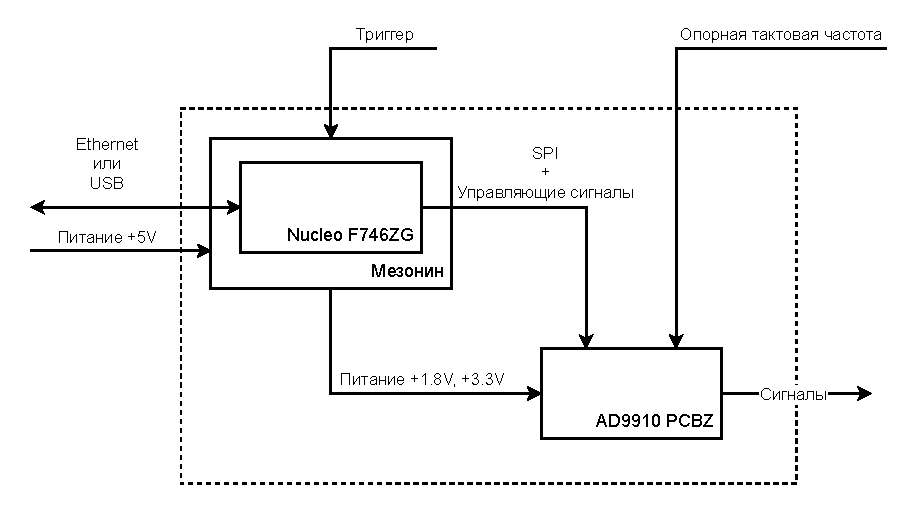
\includegraphics{data/system_architecture.drawio.pdf}
\caption{Общая схема устройства.}
\label{fig:system_architecture}
\end{figure}
\end{gostfigure}

Управление устройством осуществляется c ПК по USB или Ethernet, через виртуальный ком-порт в первом случае и через утилиту netcat во втором случае. Устройство предоставляет текстовый интерфейс, который включает в себя комманды добавления сигналов в очередь, очистки очереди, запуска и остановки воспроизведения из очереди.

\pagebreak

Триггер может предоставлятся как внешним устройством, так и самим микроконтроллером: на мезонинной плате предусмотрена перемычка, которая позволяет выбирать внешний либо внутренний источник. Частота следования триггеров может варьироваться в разумных пределах; внутренний источник сконфигурирован под стробирующий сигнал с частотой 25 Гц.

Ниже представлено схематичное изображение процесса подачи сигналов, схожее с тем, что можно было бы увидеть на осциллоскопе:

%
% Схематичное изображение процесса работы
%
\begin{gostfigure}
\begin{figure}[H]
\centering
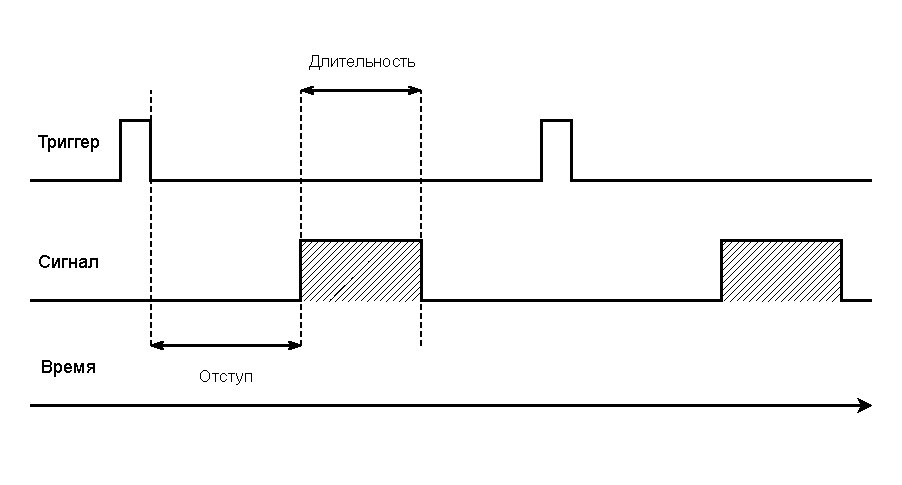
\includegraphics{data/timing_diagram.drawio.pdf}
\caption{Подача сигналов.}
\label{fig:timing_diagram}
\end{figure}
\end{gostfigure}

\subsection{Программирование}

Прошивка для микроконтроллера написана на языке программирования C, с использованием преимущественно свободных инструментов с открытым исходным кодом.

В качестве компилятора C использован gcc для ARM; все используемые в проекте библиотеки нацелены именно на этот компилятор, что и послужило главной причиной для его выбора. Возможной альтернативой является компилятор clang в составе проекта LLVM, но не проверялось, сможет ли он без ошибок собрать все задействованные библиотеки, в особенности STM32 HAL, который может содержать специфичный для gcc код.

В качестве системы сборки использован GNU Make. Задача Make состоит в запуске команд сборки, также называемых правилами, для каждого файла с исходным кодом. Главное преимущество от использования Make по сравнению с, например, скриптом сборки для интерпретатора командной строки, будь это bash или что-нибудь другое, заключается в возможности параллельной сборки, когда не зависящие друг от друга файлы с исходным кодом собираются параллельно, что позволяет существенно ускорить полную сборку проекта. Другим преимуществом является поддержка частичной сборки, когда повторно компилируются только файлы, изменившиеся с момента предыдущей сборки. Нужно отметить, что существуют и другие системы сборки, например CMake и ninja, которые обладают схожими возможностями, но часто сложнее в использовании.

В качестве IDE использована среда разработки VSCode, которая была выбрана преимущественно в связи с её популярностью и наличием расширения C/C++ IntelliSense, которое предоставляет быстрый поиск идентификаторов во всех файлах проекта и является незаменимым инструментом при изучении кода больших библиотек, таких как STM32 HAL. Нужно отметить, что, в отличие от самого VSCode, это расширение не является полностью свободным — его исходный код закрыт. Другими IDE, которе бы подошли для разработки прошивки под ARM устройство, являются Qt Creator и CLion.

В качестве инструмента для загрузки собранной прошивки в микроконтроллер а также отладки использован OpenOCD. Этот инструмент позволяет прошивать множество микроконтроллеров от разных производителей а также выступает сервером отладки для gdb.

Наконец, в качестве отладчика использован gdb, который не имеет возможности самостоятельно взаимодействовать с отлаживаемым устройством и полагается на OpenOCD в качестве сервера.

\subsection{Использование AD9910}

Цифровой синтезатор сигналов (DDS) AD9910 представлен в исполнении производителя на отладочной плате AD9910 PCBZ. Данная плата предусматривает управление при помощи внешнего микроконтроллера через выведенные на контактные гребенки входы и выходы, либо с ПК при помощи интерфейса USB, который реализован неизвестным микроконтроллером на плате.

Ниже представлены некоторые ключевые характеристики AD9910:

\begin{itemize}
	\item Максимальная внутренняя частота: 1 ГГц.
	\item Разрядность ЦАП: 14 бит.
	\item Восемь профилей частоты, амплитуды и начальной фазы сигнала, между которыми возможно быстрое переключение.
	\item Параллельный порт для быстрого изменения одного из параметров сигнала.
	\item Внутренняя оперативная память для сложных сигналов.
\end{itemize}

% TODO: Объяснить в теоретической части, что чем выше тактовая частота DDS, тем больше точность аппроксимации
Для работы AD9910 требуется источник тактовой частоты, которым может выступать кварцевый резонатор на плате или внешний генератор. В случае использования внешнего генератора, есть три способа получения максимальной внутренней частоты: AD9910 может работать на прямую от поступающей от внешнего источника частоты, либо может делить её на два через встроенный делитель или умножать на число от 12 до 127 при помощи встроенного PLL (Блока ФАПЧ); это позволяет использовать внешние частоты, равные 1 ГГц, 2 ГГц или $\frac{1}{x}$ ГГц, где $12 \leq x \leq 127$ и $x$ является целым. Для первичной проверки работоспособности синтезатора использовалась внешняя частота равная 200 МГц и AD9910 работал на сниженной скорости.

В режиме управления с ПК, синтезатор подключается по USB, и используя утилиту от производителя (представлена на рисунке \ref{fig:ad9910_evaluation_software}) можно управлять всеми его настройками, видя при этом изменения в содержимом регистров. Это крайне полезный инструмент для ознакомления с устройством.

\begin{gostfigure}
\begin{figure}[H]
\centering
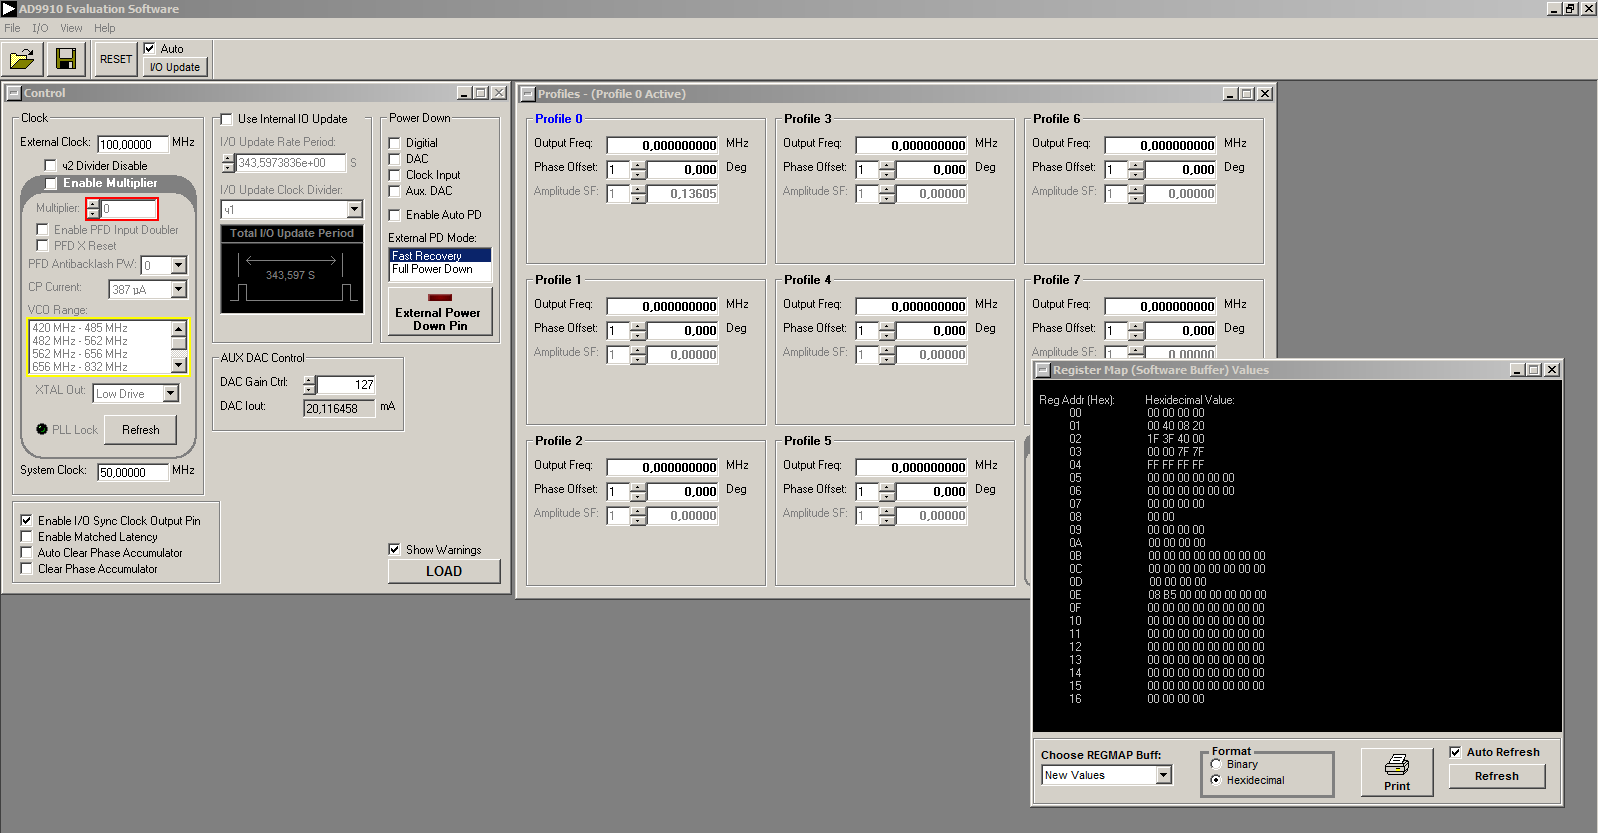
\includegraphics[scale=.25]{data/ad9910_evaluation_software.png}
\caption{Утилита управления синтезатором AD9910 с ПК.}
\label{fig:ad9910_evaluation_software}
\end{figure}
\end{gostfigure}

Всего синтезатор имеет 23 регистра с различной шириной, от 2 байт до 8 байт. В большинстве случаев, один бит регистра отвечает за включение/выключение определённой функции синтезатора, но есть некоторые регистры, которые отведены под хранение числовых значений, например регистры 15–22 используются для хранения восьми профилей генерируемой частоты. Полное описание полей регистров чипа AD9910 можно найти в источнике \cite{AD9910Datasheet}.

Расположенный на плате синтезатора микроконтроллер не подходит для решения поставленной задачи по двум причинам: во-первых, у него нет интерфейса Ethernet, а это является одним из требований к устройству. Во-вторых, исходные коды его существующей прошивки нигде не доступны. Поэтому встроенный микроконтроллер был отключен перестановкой перемычек на плате.

Управление внешним микроконтроллером осуществляется при помощи множества выделенных под отдельные функции синтезатора управляющих сигналов а также SPI для доступа к регистрам.

Используемые для SPI входы и выходы представлены в таблице \ref{tab:spi_pins}:

% %%%%%%%%%%%%%%%%%%%%%%%%%%%%%%%%%%%%%%%%%%%%%%%%%%%%
% Таблица используемых для SPI входов и выходов AD9910
% %%%%%%%%%%%%%%%%%%%%%%%%%%%%%%%%%%%%%%%%%%%%%%%%%%%%
\begin{table}[H]
\centering
\caption{Используемые для SPI входы и выходы AD9910}
\label{tab:spi_pins}
\begin{tabular}{|p{4cm}|p{8cm}|}
\hline 
\textbf{Название} & \textbf{Пояснение} \\ 
\hline 
CSB & Низкий уровень на этом входе активирует порт SPI синтезатора \\ 
\hline
SCLK & Тактовый сигнал SPI подаваемый устройством-мастером \\
\hline
SDO & Выход SPI для отправки данных устройству-мастеру \\
\hline
SDIO & Вход SPI для получения данных от устройства-мастера, или вход и выход одновременно, в зависимости от выбранного режима SPI \\
\hline 
IO\_RESET & Высокий уровень на этом входе отменяет текущую транзакцию \\
\hline
\end{tabular} 
\end{table}

В рамках одной транзакции данных синтезатору сначала отправляется инструкция размером в один байт, где старший бит выбирает между режимом записи и режимом чтения, а пять младших битов определяют номер интересующего регистра. В режиме записи должны последовать {\em n} байт, где {\em n} — ширина регистра, а в режиме чтения, наоборот, должно быть считано {\em n} байт.

Значения, записанные в регистры синтезатора, вступают в силу не сразу. Изначально они находятся в буфере ввода-вывода, и чтобы скопировать их в действующие регистры, нужно подать импульс высокого уровня на линию IO\_UPDATE, либо изменить состояние входов выбора профиля.

Для начального запуска синтезатора под управлением микроконтроллера был использован подход с записью всех регистров эталонными значениями: благодаря утилите производителя, мы знали, какое в точности содержимое должно быть в каждом регистре синтезатора для получения непрерывного сигнала на некоторой частоте. Так как внутреннее состояние синтезатора представлено только его регистрами, можно просто перезаписать содержимое всех регистров этими заранее известными значениями, и, при прочих равных условиях, синтезатор начнёт генерировать сигнал на выходе. Здесь мы столкнулись с первой проблемой: изначально синтезатор совершенно не хотел работать под управлением микроконтроллера, не отвечая на запросы по шине SPI и не выдавая никаких сигналов даже после записи всех необходимых регистров вслепую. Мы несколько раз переключали его обратно в режим управления с ПК, что подразумевает перестановку нескольких перемычек на его плате, чтобы убедиться, что он всё ещё работает.

Наше первое предположение заключалось в том, что мы как-то неправильно настроили шину SPI на микроконтроллере. Мы попробовали множество различных комбинаций скоростей, полярностей и фаз, безрезультатно.

Мы потратили много времени на изучение сигналов на плате при помощи осциллоскопа, пытаясь найти какие-нибудь различия в сигналах на плате при работе в режиме управления с ПК и в режиме управления с микроконтроллера. Прослушивание шины SPI при отправке команд из утилиты производителя позволило нам точно определить необходимые параметры SPI—мы предположили, что продолжительность либо порядок управляющих сигналов, которые мы подаём с микроконтроллера, не соответствует спецификациям AD9910. Мы привели все задержки к абсолютно безупречному виду на осциллоскопе, но синтезатор всё равно не работал.

Единственной зацепкой, которую мы нашли, было следующее: когда плата сконфигурирована под управление микроконтроллером, исчезает сигнал в гнезде SYNC\_CLK, который иначе присутствует после первого запуска утилиты производителя и составляет ¼ частоты внешнего источника. Это навело нас на мысль, что мы пытаемся отправлять чипу AD9910 команды, когда он находится в состоянии, в котором он не готов их получать.

Третье предположение заключалось в том, что мы имеем дело с какой-то электрической проблемой. Удаление перемычек, которые включают режим управления с ПК, может менять электрические характеристики на плате, например, некоторые ножки чипа AD9910 могут оказаться в неопределенном состоянии, когда раньше они были подтянуты к нулю.

В итоге это и оказалось источником проблемы—сигналы MASTER\_RESET и EXT\_PWR\_DWN, которые отвечают за общий сброс чипа и переход в спящий режим соответственно, переходили в неопределенное состояние. Этого было достаточно, чтобы чип не запускался. Нам даже не потребовалось давать высокие уровни на эти входы, достаточно было подтянуть их к нулю, после чего плата начала надежно запускаться, выдавая ожидаемый сигнал в SYNC\_CLK.

После этого чип действительно начал реагировать на команды, которые мы отправляем ему. Мы смогли понаблюдать за изменениями, происходящими от переключения отдельных битов в регистрах. Поставив перемычки между GND и входами P\_0, P\_1 и P\_2, которые отвечают за выбор профиля, чтобы привести их из неопределённого состояния к низкому уровню и принудительно выбрать нулевой профиль, и записав заранее заготовленные значения в регистры профилей, мы смогли, наконец, получить сигнал на выходе синтезатора.

Мы смогли успешно переключить синтезатор в трёхпроводной режим SPI и получили возможность считывать содержимое регистров. Теоретически, использование двухпроводного режима тоже возможно, но используемый нами микроконтроллер имеет некоторые проблемы с размером считываемых данных в этом режиме, поэтому трёхпроводной режим предпочтителен.

% Реализовано в:
% - https://github.com/AXKuhta/stm32_ad9910/commit/272f2d1457d6abef2580f479caacd4918fd27638
% - https://github.com/AXKuhta/stm32_ad9910/commit/0c8fbba4f038878d401e76cec10e339cd68cf210
Уход от записи полностью фиксированных значений в регистры синтезатора стал следующим шагом. Были реализованы функции для изменения частоты и амплитуды профилей в хранящейся памяти микроконтроллера копии содержимого регистров, затем в текстовом интерфейсе была реализована команда test\_tone, которая принимает в качестве аргумента частоту.

Режим выдачи тона на фиксированной частоте полезен при изучении качества генерируемого сигнала при помощи анализатора спектра, где, как правило, требуются непрерывный сигнал. Анализаторы спектра могут показать наличие шумов и гармоник, которые неизбежно будут присутствовать в генерируемом DDS сигнале. Также режим фиксированного тона можно использовать, чтобы убедиться, что PLL синтезатора установился на требуемой частоте. Между двумя сигналами, первый из которых создаётся синтезатором, а второй создаётся другим генератором, работающим от того же источника опорной тактовой частоты, не должно наблюдаться смещения волн относительно друг друга при просмотре на осциллоскопе. Здесь нужно иметь ввиду, что должна быть выставлена частота, которую можно получить делением внутренней частоты синтезатора на степень двойки, поскольку DDS могут генерировать только такие частоты с абсолютной точностью.

Говоря про PLL, следующим шагом после получения сигнала из синтезатора стало задействование блока PLL, чтобы начать использовать синтезатор на полной скорости путём умножения опорной частоты.

Блок PLL в AD9910 состоит из нескольких регулируемых напряжением источников частоты (VCO), предназначенных для работы в разных диапазонах частот. Из всех VCO выбирается тот, в диапазон которого попадает требуемая внутренняя частота синтезатора. Так как мы хотим использовать синтезатор на его максимальной тактовой частоте, мы выбираем самый быстрый VCO. Принцип работы ФАПЧ (PLL) заключается в измерении расхождения между частотой VCO, разделённой на некоторое число, и опорной частотой. Расхождение используется, чтобы регулировать напряжение VCO для минимизации ошибки в частоте, и в результате обратной связи VCO достаточно быстро устанавливается на требуемой частоте. В целом, VCO в блоке PLL может работать и без опорной частоты, но тогда внутренняя частота синтезатора определена лишь примерно. Если не рассматривать PLL в деталях, то проще думать о нём, как о некотором компоненте синтезатора, который может осуществлять умножение опорной тактовой частоты на множители в диапазоне $12\times$--$127\times$. Выбор множителя осуществляется изменением полей в регистрах, после чего PLL включается установкой соответствующего бита.

Здесь была встречена следующая проблема: при использовании PLL, сигнал на выходе синтезатора приобретал крайне нестабильный характер. На выходе PLL\_LOCK, который должен сигнализировать, что PLL установился на нужной частоте, сохранялся низкий уровень. Причина заключалась в том, что для использования PLL требовалось установить на плату синтезатора несколько дополнительных компонентов, которые образуют низкочастотный фильтр, который сглаживает сигнал ошибки и необходим для правильной работы PLL. Что интересно, обязательность этих компонентов была явным образом обозначена в инструкции к отладочной плате, но не в даташите от AD9910. Производитель предоставляет построенный в виде таблицы для MS Excel инструмент (PLL Loop Filter Tool), который позволяет вычислить наиболее подходящие для используемой опорной частоты номиналы компонентов фильтра, что и было сделано. Руководствуясь полученными в результате вычислений значениями, на плату синтезатора были установлены компоненты,сконфигурировавшие её под опорную частоту, составляющую примерно 20 МГц. Это помогло разрешить проблему---на выходе PLL\_LOCK начал возникать высокий уровень, и сигнал на выходе синтезатора стал стабильным. Данный момент был важен, так как синтезатор впервые заработал на своей полной внутренней частоте в 1 ГГц.

Управление состоянием входов профилей на синтезаторе стало следующей задачей. Возможность быстро изменять все три параметра сигнала посредством профилей позволяет реализовать модуляцию. Например, можно использовать два профиля с одинаковой частотой и амплитудой, но различающейся на 180° фазой, чтобы реализовать модуляцию BPSK. Были убраны поставленные ранее перемычки и входы P\_0, P\_1 и P\_2 были подключены к микроконтроллеру. Для получения контроля амплитуды через профили также потребовалось включить в регистрах бит Enable Amplitude Scale from Single Tone Profiles, который почему-то выключен по умолчанию; пока этот бит выключен, амплитуда для всех профилей общая и берётся из вторичного регистра.

Наконец, мы подошли к самой главной проблеме использования синтезатора: формирование импульсов вместо непрерывных сигналов. Для этого требуется реализовать прекращение и возобновление подачи сигнала, и существует несколько разных способов сделать это на AD9910. Даташит не рассматривает конкретный сценарий использования с формированием импульсов и следовательно не содержит информации о том, какой из подходов лучше.

Первый подход состоит в использовании нулевой амплитуды в одном из профилей. Включение такого профиля приведёт к тому, что независимо от остального состояния синтезатора, после блока масштабирования по внутренней шине данных на АЦП будут поступать только нули, и сигнала на выходе не будет. Недостаток этого метода заключается в том, что один профиль потребуется навсегда зарезервировать как "парковочный" профиль, и для модуляции останутся доступны только семь профилей, что сделает невозможным создание некоторых видов модуляции, например 8-PSK, хотя, как обнаружилась позднее, модуляция 8-PSK при помощи профилей всё равно невозможна из-за другой проблемы, которую не получилось решить.

Второй подход заключается в использовании блока OSK в синтезаторе, который предназначен для управления амплитудой и может достичь схожего эффекта с применением нулевой амплитуды к сигналу в зависимости от уровня на выделенном входе OSK. Недостаток OSK заключается в том, что он имеет наибольший возможный приоритет в качестве источника амплитуды в синтезаторе, и когда он включен, пропадает возможность использовать амплитуду из профилей или оперативной памяти, что очень критично. Из-за этого было решено вообще не использовать OSK и не подводить его управляющий вход к микроконтроллеру.

Третий подход заключается в использовании статического сброса накопителя фазы в сочетании с режимом вывода синусоиды---двух возможностей, которые доступны через регистры синтезатора. Как и в предыдущем способе, это приведёт к поступлению исключительно нулей по внутренней шине данных на АЦП и отсутствию сигнала на выходе. Главная проблема с этим подходом состоит в том, что потребуется больше времени, чем с переключением профилей, так как необходимо произвести запись одного регистра по SPI, затем подать высокий уровень на вход IO\_UPDATE для применения изменений, что далее обозначается как "выполнить IO\_UPDATE."

Четвертый подход заключается в использовании входа EXT\_PWR\_DOWN для отправки синтезатора в режим пониженного энергопотребления с быстрым восстановлением, когда все блоки синтезатора кроме PLL отключаются. Здесь не имеет значения состояние внутренней шины данных, так как АЦП отключается по настоящему. Несмотря на то, что таким образом действительно можно прекратить подачу сигналов, данный метод не подойдёт для наших целей, так как он также отключает порт SPI и убирает возможность изменить регистры синтезатора в промежутке между импульсами.

% Реализовано в:
% - https://github.com/AXKuhta/stm32_ad9910/commit/2e487a1fa9ddbbce861b1afd3613c8091fd185eb
В итоге был выбран первый способ, когда нулевой профиль зарезервирован под прекращение подачи сигнала и режим ожидания триггера. Для начала подачи сигнала происходит переключение на другой профиль с ненулевой амплитудой. В изначальной реализации переключение профиля осуществлялось из контекста прерывания на микроконтроллере, с достаточно большим разбросом по времени. Позднее, для установки уровней на входах профилей был задействован DMA, что позволило уменьшить разброс.

У этого подхода присутствует одна проблема: непредсказуемая начальная фаза сигнала. Включение профиля с нулевой амплитудой и нулевой частотой уберёт сигнал с выхода и остановит изменение значения в накопителе фазы, но накопитель не будет сброшен, и в этом кроется проблема: в момент начала следующего импульса старое значение фазы приведёт к началу сигнала со значения синуса в произвольной точке, а не в нуле, что будет выглядеть на осциллоскопе как резкий прыжок или резкий провал, после которого начинает следовать нормальная синусоидальная волна. Наличие таких разрывов в сигнале нежелательно, но в целом терпимо. Из непредсказуемой начальной фазы также следует непредсказуемость фазы во всех остальных точках сигнала. Иными словами, положение пиков в синусоидальной волне на протяжении всего сигнала будет различаться между запусками, что тоже нежелательно, но терпимо, т.к. не препятствует использованию устройства для снятия АЧХ.

% https://tex.stackexchange.com/questions/168430/xelatex-polyglossia-hyphenation
Тем не менее, проблему с непредсказуемой начальной фазой можно исправить. Как уже упоминалось ранее, у синтезатора присутствует возможность статического сброса накопителя фазы, когда его значение удерживается на нуле. На самом деле, существует два способа сбросить накопленную фазу: статический сброс, который переключается битом \textenglish{Clear phase accumulator} в регистрах, и сброс при переключении профилей, который переключается битом Autoclear phase accumulator. В случае со сбросом по переключению профиля механизм работы достаточно понятен: при каждом изменении состояния входов профилей, фаза сбрасывается. Для сигналов, в которых отсутствует модуляция при помощи профилей, можно без опаски использовать этот способ сброса фазы, так как профиль будет переключаться только в начале и в конце сигнала, и никогда не будет переключаться посередине. Если же используется модуляция при помощи профилей, то использование Autoclear phase accumulator приведёт к сбросу фазы в моменты смены элементов кода, создавая разрывы в сигнале, а в случае с PSK модуляцией вообще затруднит использование, т.к. этот вид модуляции полагается на сдвиг фазы относительно предыдущего значения, а не переход на абсолютное значение. В этом случае лучше подойдёт статический сброс фазы, принцип работы которого несколько сложнее: при включении бита Clear phase accumulator, накопитель фазы принудительно удерживается в сброшенном состоянии, т.е. всегда равен нулю и не увеличивается.

% TODO: Диаграмма
% Рисунок 1: с произвольной начальной фазой
% Рисунок 2: с нулевой начальной фазой
Чтобы начать подачу сигнала из этого состояния, нужно выключить статический сброс до начала подачи следующего сигнала и вызвать применение изменений, выполнив IO\_UPDATE. После выключения статического сброса, если выбран профиль с нулевой частотой, то значение накопителя не начнёт увеличиваться и по шине данных на ЦАП продолжат поступать нули. Затем, когда будет включен профиль с ненулевой частотой, значение накопителя фазы начнёт расти с нуля и на выходе получится сигнал с предсказуемой начальной фазой. Здесь стоит вспомнить, что применение изменений в регистрах происходит не только от IO\_UPDATE, но и от переключения профилей, так что применение IO\_UPDATE после отключения статического сброса необязательно, т.к. изменения всё равно будут применены в момент включения нового профиля.

Позднее, когда была реализована подача сигналов с произвольными кодовыми последовательностями и FSK/PSK модуляцией при помощи переключения входов профилей, обнаружилась существенная проблема: при одновременном изменении состояния на более чем одном входе P\_x, например при одновременном выставлении высокого уровня на P\_0 и P\_1, синтезатор может выбрать неправильный профиль: несмотря на то, что был выбран профиль 3, с некоторой вероятностью может быть включен как профиль 3, так и профиль 1 либо профиль 2. Точная причина такого поведения не ясна, но скорее всего дело в отсутствии синхронизации переключения профиля относительно тактового сигнала SYNC\_CLK, который внутренне отвечает за опрос всех интерфейсов синтезатора. В даташите явно указано, что уровни на входах профилей должны быть установлены не менее чем за 1.75 нс до переднего фронта SYNC\_CLK, но в текущей реализации это требование не соблюдено и уровни на входах профилей устанавливаются в совершенно произвольные моменты времени относительно SYNC\_CLK. В результате, синтезатор правильно воспринимает только изменение состояния одного входа профилей за один период SYNC\_CLK. Было решено оставить всё так, поскольку это не препятствует реализации подачи сигналов без модуляции или с простой модуляцией, где не требуется переключать более одного входа профилей за раз, например в BPSK.

% TODO: Диаграмма отсчёта DRG вверх
Ранее, была также реализована линейно-частотная модуляция (ЛЧМ) с использованием блока DRG в AD9910. Блок DRG представляет из себя 32-х битный счётчик, выходное значение которого можно использовать в качестве параметра частоты, амплитуды или фазы сигнала, хотя в случае с амплитудой и фазой задействованы только 16 и 14 младших бит соответственно. Двумя основными параметрами DRG являются значения инкремента и декремента, которые также можно понимать как величину шага по частоте в случае использования DRG в качестве источника значения частоты. Выбор между применением инкремента и декремента, и, соответственно, растущим или убывающим итоговым значением определяется состоянием входа DR\_CTL, где высокий уровень соответствует выбору инкремента, а низкий уровень выбору декремента. Другим ключевым параметром является значение темпа (Ramp Rate) выполнения шагов, которое внутренне является начальным значением для отсчитывающего до нуля таймера. Более высокие значения Ramp Rate соответствуют большему интервалу между шагами, а минимальным полезным значением является 1, когда интервал выполнения шагов составит 4 нс при внутренней частоте AD9910 в 1 ГГц; шагов не будет происходить вообще, если записать ноль в регистр Ramp Rate. Помимо инкремента, декремента и интервала между шагами, можно задать нижнюю и верхнюю границу для выходного значения. Нижняя граница всегда берётся в качестве начального значения счётчика.

Ниже представлено схематичное изображение спектра сигналов, которые можно получить с определёнными параметрами DRG. Для наглядности выбран чрезвычайно большой шаг по частоте $a$, в то же время интервал шагов $b$ и общая длительность подобраны для получения сигнала с всего тремя частотными составляющими.

%
% Некоторые частные случаи ЛЧМ сигналов
%
\begin{gostfigure}
\begin{figure}[H]
\centering
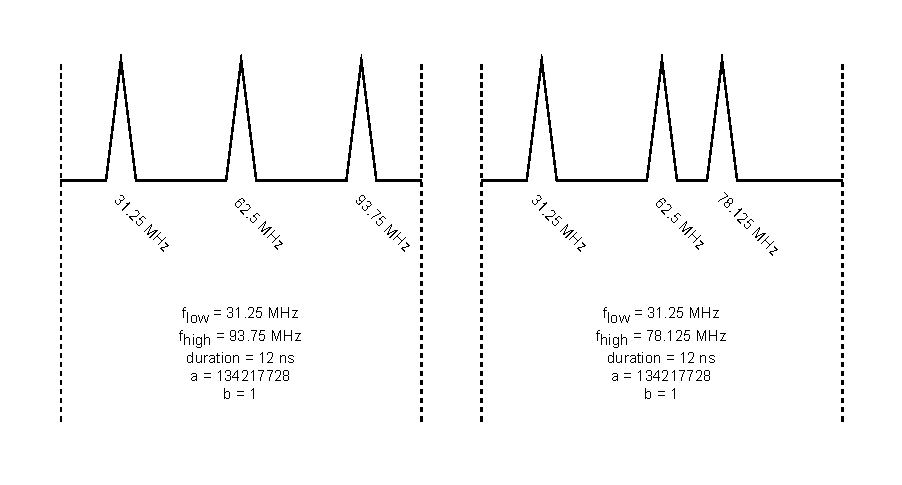
\includegraphics{data/sweep_edge_cases.drawio.pdf}
\caption{Некоторые частные случаи ЛЧМ сигналов.}
\label{fig:sweep_edge_cases}
\end{figure}
\end{gostfigure}

Как можно заметить на рисунке справа, разница по частоте между последней и предпоследней частотными составляющими в ЛЧМ сигнале может быть меньше изначально заданного шага по частоте в связи с тем, что значение верхней границы частоты обладает приоритетом. Конечно, в реальности синтезатор будет использоваться для создания сигналов с гораздо более высокой плотностью частотных составляющих, где дискретизирующие АЦП буквально не смогут увидеть разницы, и выделять отдельные частоты не будет смысла.

Рассмотрим ЛЧМ сигнал с длительностью в 900 мкс с параметрами $a=1, b=1$: если AD9910 работает с тактовой частотой 1 ГГц, то за 900 мкс DRG сможет сделать 225000 шагов, но последний шаг будет сделан ровно в момент прекращения подачи сигнала, так что мы имеем дело с изменением начальной частоты на 224999 инкрементов, значение каждого из которых составляет примерно 0.232 Гц, следовательно полоса ЛЧМ сигнала составит примерно 52.386 кГц.

По сравнению с подачей сигналов с фиксированной частотой, подача ЛЧМ сигналов требует дополнительных действий в момент начала подачи сигнала. Во-первых, счётчик DRG должен быть сброшен; для этого доступно два механизма, схожих по принципу действия с механизмами сброса аккумулятора фазы: это сброс по событию, либо статический сброс. Включение статического сброса приведёт к удержанию счётчика в сброшенном состоянии, где значение равно нижней границе. При использовании сброса по событию, изменение состояния входов профилей либо применение IO\_UPDATE приведёт к сбросу счётчика на нижнюю границу. Во-вторых, должен быть сброшен таймер шагов. Он всегда сбрасывается при изменении состояния на входе DR\_CTL, а также может сбрасываться по событию, если выставлен бит Load LRR @ IO Update. В текущей реализации используется сброс счётчика и таймера по событию, что не позволяет использовать модуляцию профилями (в данном случая для изменения амплитуды или фазы) при подаче ЛЧМ сигналов, но модуляция при помощи оперативной памяти остаётся возможной.

Особым случаем является подача ЛЧМ сигналов, где начальная частота выше конечной. Так как стандартными средствами можно произвести сброс только на нижнюю границу, возникает вопрос: как начать ЛЧМ сигнал с верхней границы? Возможным решением является запись значения начальной частоты в регистры нижней и верхней границы одновременно, и выполнение сброса по событию, что должно привести к записи и удержанию значения начальной частоты в счётчике, после чего можно записать значение конечной частоты в регистр нижней границы и применить изменения без сброса. После этого, при смене уровня на вход DR\_CTL на низкий, DRG должен отсчитывать от верхней границе к нижней границе. Данный метод не испытывался, поскольку даташит явно требует, чтобы значение в регистре верхней границы было больше значения в регистре нижней границы, а запись одинаковых значений нарушила бы это условие.

Другим возможным решением является запись значения $2^{32}-1$ в регистр инкремента, что является максимальным возможным значением, выполнение сброса по событию, и ожидание в течение четырёх тактов синтезатора, после чего счётчик выполнит один отсчёт и начнёт удерживать значение верхней границы вместо значения инкремента. Затем, при смене уровня на входе DR\_CTL на низкий в момент начала сигнала, счётчик начнёт отсчитывать с верхней границы к нижней границе. Данный метод тоже не испытывался.

Наконец, ещё одним возможным решением является использование зеркальных частот, которые получаются при значениях $FTW > 2^{31}$ и были рассмотрены в теоретической части этой работы. Так как смысл таких значений $FTW$ меняется, и большие значения соответствуют меньшим частотам, возникает возможность использовать меньшее значение, соответствующее большей начальной частоте, в качестве нижней границы, и наоборот, использовать значение с меньшей частотой в качестве верхней границы. Главной особенностью такого режима работы синтезатора является то, по своему наблюдаемому поведению аккумулятор фазы становится обратным счётчиком, и генерация синусоиды начинается с конца, что выглядит на осциллоскопе как повёрнутая на 180 градусов фаза, что, к счастью, легко компенсируется. В итоге для подачи ЛЧМ сигналов с убывающей частотой был выбран именно этот способ.

% TODO: Свип от высокой частоты к низкой
% TODO: FMCW
% TODO: Диаграмма с неудачным свипом

\section*{ЗАКЛЮЧЕНИЕ}
bbb

% Список литературы.
\begin{thebibliography}{11}
\bibitem{DDSTutorial} A Technical Tutorial
on Digital Signal Synthesis https://www.ieee.li/pdf/essay/dds.pdf
\bibitem{AD9910Datasheet} Analog Devices, AD9910 Datasheet
\bibitem{Kushnarev} Кушнарев Д.С., Лебедев В.П., Хахинов В.В., Евстифеев С.Е., Заруднев В.Е. Модернизация Иркутского радара некогерентного рассеяния. Солнечно-земная физика. 2017. Т. 3, № 3. С. 88-94.
\end{thebibliography}

\appendix

\begin{gostappendix}{Программный код}
\lstset{language=[11]c++,basicstyle=\ttfamily, showstringspaces=false}

\begin{lstlisting}
#include <iostream>

using namespace std;

int main()
{
  auto b = 1;
  auto a = 2;
  cout << "2 + 1 = " << a + b << endl;
  return 0;
}
\end{lstlisting}
\end{gostappendix}


\begin{gostappendix}{Таблица}
aaa
\end{gostappendix}


\end{document}
